\subsection{Printplaten}
Nu dat alle schakelingen zijn ontworpen moeten deze ook nog fysiek in elkaar gezet kunnen worden. Omdat een aantal componenten enkel in surface mount packages verkregen kunnen worden zal er een PCB ontworpen moeten worden. Om het testen te vereenvoudigen is er voor gekozen om de voeding op een tweede PCB te implementeren, los van de rest van het \si{\pH} meetsysteem.

Er zal een twee tal connectoren op beide PCB's worden geplaatst zodat de ISFET uitlees en communicatie PCB uiteindelijk gevoed kan worden door de voeding PCB. Een van de twee connectoren zal enkel gebruikt worden om te voeden en de tweede connector kan gebruikt worden voor communicatie tussen de twee PCB's.

Er zal eerst ingegaan worden op het ontwerp van de ISFET uitlees en communicatie PCB. Dit wordt opgevolgd door het ontwerp van de voeding PCB.
% De schakelingen voor de voeding en voor het uitlezen van de ISFET zijn opgedeeld in twee verschillende printplaten. Dit is gedaan zodat beide schakelingen apart van elkaar getest kunnen worden. De uitlees PCB is te zien in \cref{fig:sensorPCB}. Deze PCB bevat de ISFET uitleesschakeling en de \mcu, die de gemeten pH waarde naar het basisstation opstuurt. De voeding printplaat is te zien in \cref{fig:powerPCB}. Deze PCB regelt de energy harvesting, samen met het veilig opladen en het ontladen van de batterij. De twee printplaten zijn met elkaar verbonden door middel van pin headers. Beide schakelingen zijn te zien \cref{fig:PCBs}.

% Beide PCB's hebben op elk belangrijk signaal een testpunt. Op deze manier kan er eenvoudig gemeten worden.


% \begin{figure}[!htbp]
%     \centering
%     \begin{subfigure}[b]{0.48\textwidth}
%         \centering
%         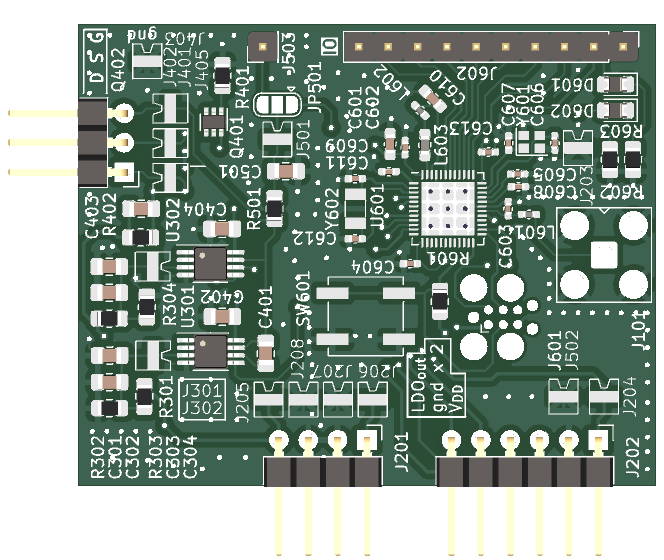
\includegraphics[width=\textwidth]{sensorBord}
%         \caption{De ISFET uitlezende PCB.}
%         \label{fig:sensorPCB}
%     \end{subfigure}
%     \hfill
%     \begin{subfigure}[b]{0.60\textwidth}
%         \centering
%         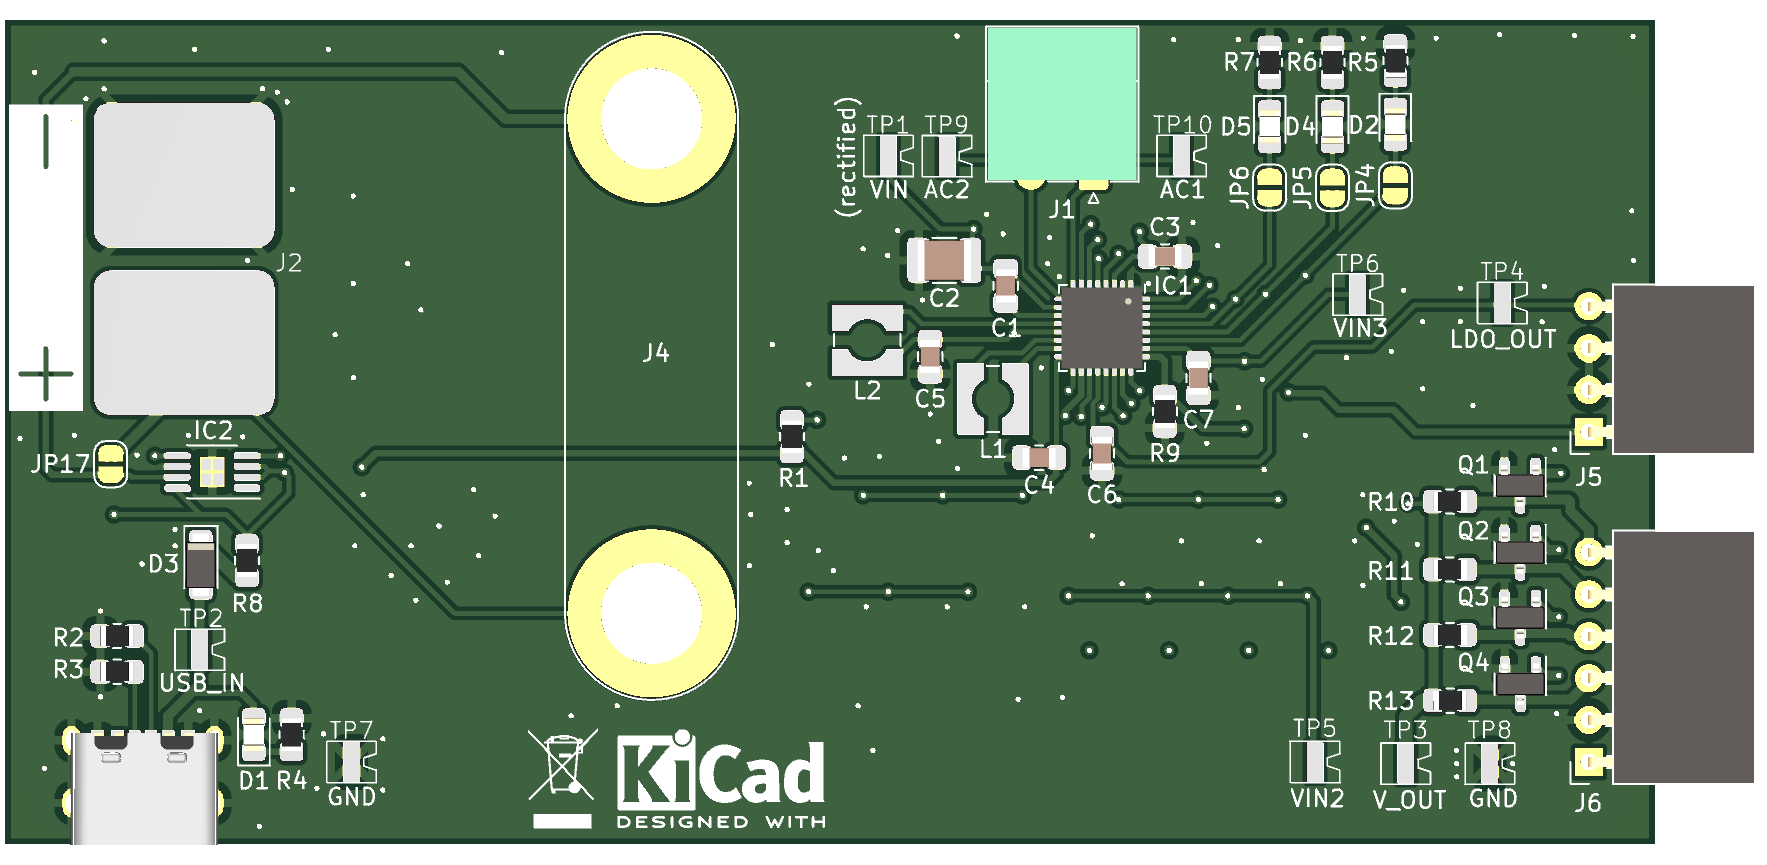
\includegraphics[width=\textwidth]{powerandharvest}
%         \caption{De voeding en harvesting PCB.}
%         \label{fig:powerPCB}
%     \end{subfigure}
%     \caption{De gemaakte PCB's.}
%     \label{fig:PCBs}
% \end{figure}

\subsubsection{ISFET uitlees en communicatie PCB}
Om de kosten van de ISFET en communicatie PCB's laag te houden is er voor gekozen om het PCB 40 bij \qty{50}{\milli\meter} te ontwerpen. Om er voor te zorgen dat

\subsubsection{Voedings PCB}

